
% ----------------------------- %
% Section 1
% ----------------------------- %
\section*{How?}

First thing I did when I looked at this
problem was to list everything I can remember
about this problem. What did we learn in Unit 5?
In Lesson 21, we learned that power series
"can be integrated term by term." In Lesson 22, 
we learned that $ sinx $ is a Taylor series, 
which in turn tells us that $ sinx $
is also a power series
because a Taylor
series is also a power series at the same time.
Thus, here's what I thought: we're going to
find how to represent
this problem in the form
of a Taylor series, and
we'll integrate that
term by term.

On the last page of our assigned reading,
which was Chapter 10.10
\textit{Applications of Taylor Series} page 640,
we learned that $ sinx $
is a frequently used
Taylor series in the
form of 
\begin{equation}
	\sum_{n=0}^{\infty}
	\frac{
		(-1)^nx^{2n+1}
	}{
		(2n+1)!
	}
\end{equation}

Let's use this to
find the Taylor series
representation of
our problem. We can
do that just by 
multiplying the above
Taylor series with 
$ \frac{1}{x} $

\begin{align}
	\textbf{19.}\quad \int_{0}^{0.1} 
	\frac{sinx}{x}\ dx
	=
    \int_{0}^{0.1} 
	\frac{1}{x}\ 
	sinx\ dx
	&=
	\int_{0}^{0.1}
	\frac{1}{x}
	\sum_{n=0}^{\infty}
	\frac{
		(-1)^nx^{2n+1}
	}{
		(2n+1)!
	}\ dx \\
    &=
   	\int_{0}^{0.1}
	\sum_{n=0}^{\infty}
	\frac{
		(-1)^nx^{2n}
	}{
		(2n+1)!
	}\ dx
\end{align}

Before diving into
the process of evaluating
the above integral,
let me quickly describe
what the overall process
of solving this problem would
look like. We'll first 
integrate term by term.
We'll be able to
approximate using
the Alternating Series
Estimation Theorem, and then
we'll verify our answer
by plotting $ \frac{sinx}{x} $
on a graph and then looking
at its area.

\newpage

% ----------------------------- %
% Section 2
% ----------------------------- %
\section*{Steps}

\begin{align}
	\textbf{19.}\quad \int_{0}^{0.1} 
	\frac{sinx}{x}\ dx
	&=
	\int_{0}^{0.1}
	\sum_{n=0}^{\infty}
	\frac{
		(-1)^nx^{2n}
	}{
		(2n+1)!
	}\ dx \\
	&=
	\sum_{n=0}^{\infty}
	\Bigg[
	\frac{
		(-1)^nx^{2n+1}
	}{
		(2n+1)
		(2n+1)!
	}
	\Bigg]_0^{0.1} \\
	&=
	\sum_{n=0}^{\infty}
	\frac{
		(-1)^n(0.1)^{2n+1}
	}{
		(2n+1)
		(2n+1)!
	} \\
	&=
	0.1 
	-
	\frac{
		0.1^{3}
	}{
	    3\cdot3!
	}
	+
	\frac{
		0.1^{5}
	}{
		5\cdot5!
	}
	-
	\frac{
		0.1^{7}
	}{
		7\cdot7!
	}
	+
	\cdots
\end{align}

% ----------------------------- %
% Section 3
% ----------------------------- %
\section*{Approximating}

Now, Alternating Series
Estimation Theorem tells us
that in an alternating series
- just like what we have above -
the greatest error value 
that its total sum can have 
is the first neglected term.
So, that's what we're gonna do.
We'll keep plugging into the
summation formula we have above,
until we find an $ n^{th} $ term
that has what our problem requires
us to have -- which is an error
of magnitude less than $ 10^{-8} $.

We could do this by using Maple too,
just so you know. 
Go to Lesson 22. 
There's a maple example file for
showing how to "approximate the value of  using a power series with an error less than 0.001"
I, however, found the $ n^{th} $ term
just by plugging in the first few values.

Here's what I got. 
$ n_3 = 0.00000001\overline{6} $
This is very close to the answer we
need, but it has 7 leading zeros, so
it's just a little bit short of what
the problem asks us to have. Thus,
going to the next term, we have
$ n_4 = 0.00000000000283\ldots $
Thus, we just found that the
summation of the first three terms
is what we're looking for. 

In conclusion, the answer to
our problem is this:

\begin{align}
	\textbf{19.}\quad \int_{0}^{0.1} 
	\frac{sinx}{x}\ dx
	&=
	0.1 
	-
	\frac{
		0.1^{3}
	}{
		3\cdot3!
	}
	+
	\frac{
		0.1^{5}
	}{
		5\cdot5!
	} \\
	&\approx
	0.09994446\overline{1}
	\ \pm  0.00000000000283
\end{align}

\newpage

% ----------------------------- %
% Section 4
% ----------------------------- %
\section*{Verification}

Here's how $ \frac{sinx}{x} $
looks like.

\begin{figure}
	\centering
	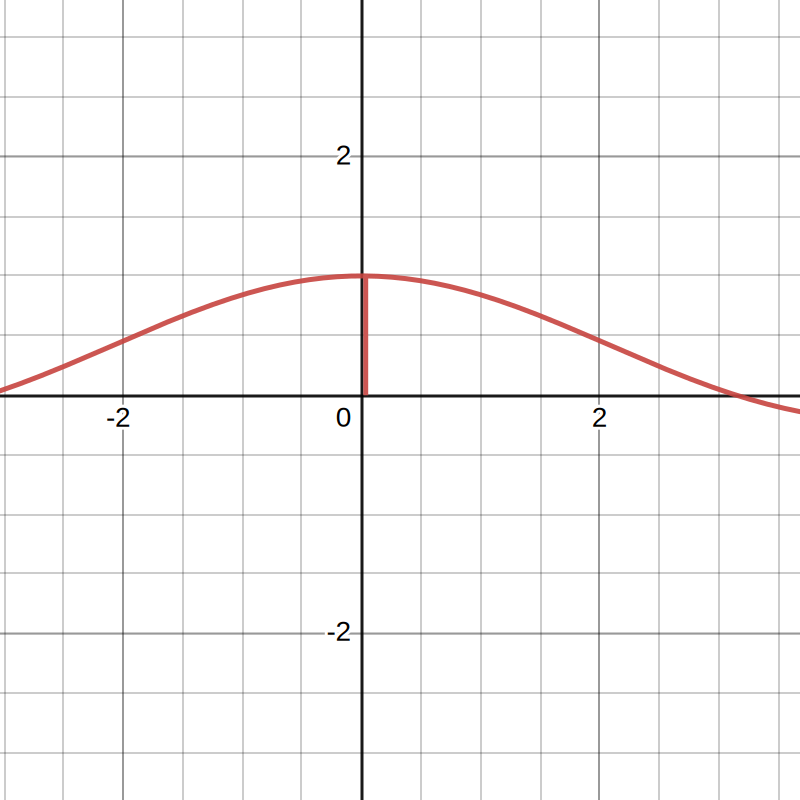
\includegraphics[width=0.43\linewidth]{verification1}
	\caption{}
	\label{fig:verification1}
\end{figure}

And here's the same graph
zoomed into the area we need.

\begin{figure}
	\centering
	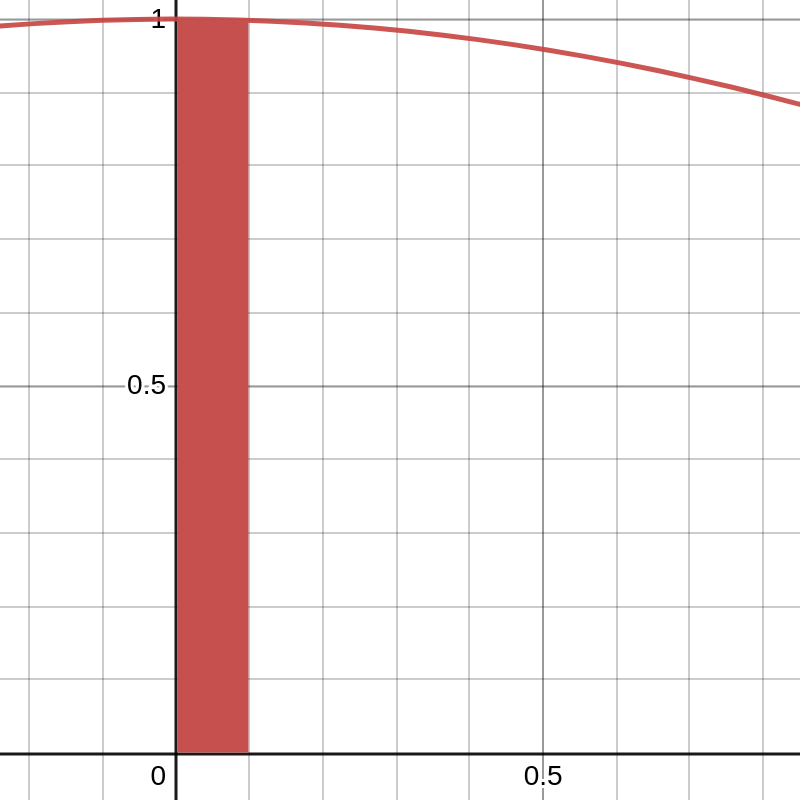
\includegraphics[width=0.43\linewidth]{verification2}
	\caption{}
	\label{fig:verification2}
\end{figure}

Approximately, the area under
the curve - the red rectangle -
has the width of
$ 0.1 $ and the height of 
around $ 1 $, which means its
area is $ 0.1 \cdot 1 \approx 0.1 $
This indeed confirms - at least
geometrically - that the answer we 
got is correct:

\begin{align}
	\textbf{19.}\quad \int_{0}^{0.1} 
	\frac{sinx}{x}\ dx
	&=
	0.1 
	-
	\frac{
		0.1^{3}
	}{
		3\cdot3!
	}
	+
	\frac{
		0.1^{5}
	}{
		5\cdot5!
	} \\
	&\approx
	0.09994446\overline{1}
	\ \pm  0.00000000000283
\end{align}


